\documentclass[11pt]{beamer}

\usetheme{metropolis}

\usepackage{graphicx}
\usepackage{physics}
\usepackage{adjustbox}
\usepackage{caption}
\usepackage{chemformula}
\usepackage{quoting}
\usepackage[style=chem-angew,backend=bibtex]{biblatex}
\bibliography{references}
%
% Choose how your presentation looks.
%
% For more themes, color themes and font themes, see:
% http://deic.uab.es/~iblanes/beamer_gallery/index_by_theme.html
%
\mode<presentation>
{
  \usetheme{default}      % or try Darmstadt, Madrid, Warsaw, ...
  \usecolortheme{default} % or try albatross, beaver, crane, ...
  \usefonttheme{default}  % or try serif, structurebold, ...
  \setbeamertemplate{navigation symbols}{}
  \setbeamertemplate{caption}[numbered]
  \setbeamerfont{footnote}{size=\tiny}
} 

\usepackage[english]{babel}
\usepackage[utf8]{inputenc}
\graphicspath{{../lectureMW/image/}}

\AtBeginSection[]{
\begin{frame}{Outline}
  \tableofcontents[currentsection]
\end{frame}
}

\title{Chapter 6: Quantities in Chemical Reactions}
\institute{Chemistry Department, Cypress College}
\date{October 6, 2022}

\begin{document}

\begin{frame}
  \titlepage
\end{frame}

\begin{frame}{Class Annoucements}
  \textbf{Lecture}
  \begin{itemize}
  \item Keep submitting the homework assignment on time
    ($\sim 1-2$ hours grace period)
  \item Go over homework 4 - present and get 1 EC point
  \item Quiz submissions are slacking (Quiz 5 due tonight
    at 11:59pm)
  \item Homework and Quiz will be released Fri, Oct 7 at 3pm
  \end{itemize}
\end{frame}

\section{Limiting Reactant/Reagent}

\begin{frame}{Application: Baking a Cake}
  \centering
  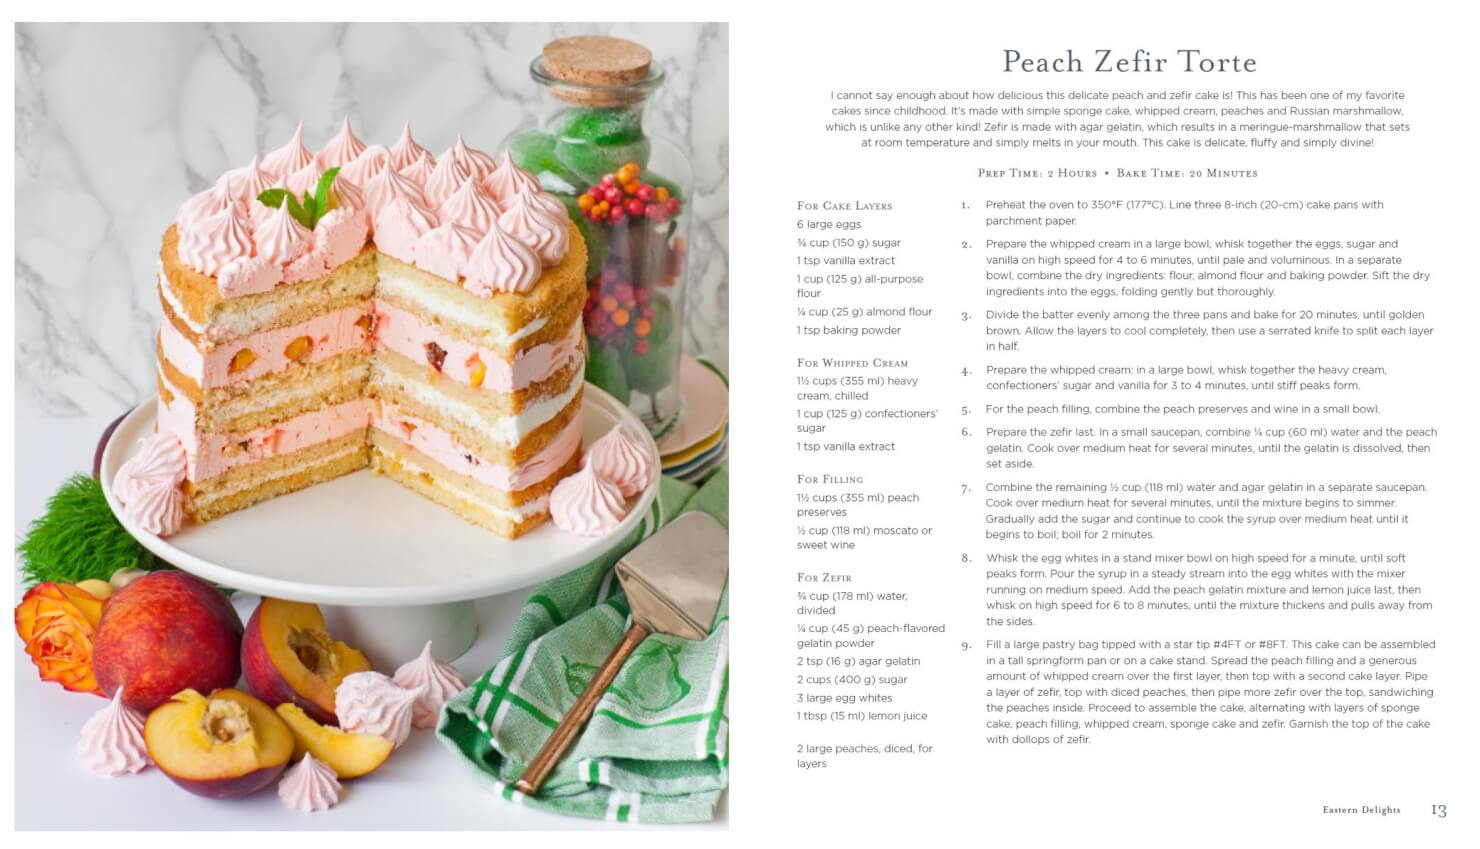
\includegraphics[width=\linewidth]{peach_cake}
\end{frame}

\begin{frame}{Approaching Limiting Reactant Problems}
  \begin{equation}
    \text{R1} + \text{R2} \rightarrow \text{P1}
  \end{equation}
  \begin{itemize}
  \item Given a certain amount of each reagents (R1 and R2)
    to produce P1, determine
    how much the R2 is needed to completely react with R1
  \item Based on that calculated value, determine whether
    there is enough R2 to completely react with R1
  \item If the amount of R2 is less than what is needed,
    then R2 is the limiting
  \item If the amount of R2 is more than what is needed,
    then R2 is the excess
  \end{itemize}
\end{frame}

\begin{frame}{Example: Limiting Reactant/Reagent}
  Ethylene, C$_2$H$_4$, undergoes many useful reactions. However,
  it is highly flammable and burns in the presence of oxygen. Suppose
  a mixture of 0.25 mol C$_2$H$_4$ and 1.0 mol O$_2$ leads to a combustion.
  Determine the limiting reactant, excess reactant and amount of CO$_2$
  formed in mols.
  
  \onslide<2->{
    C$_2$H$_4$(g) + 3 O$_2$(g) $\rightarrow$ 2CO$_2$(g) + 2H$_2$O(g)
  }
  \onslide<3->{\begin{align*}
      1.0 \text{mol O$_2$} \times \frac{1 \text{mol C$_2$H$_4$}}{3 \text{mol O$_2$}} = 0.33333 \text{mol C$_2$H$_4$}
    \end{align*}
  }
  \onslide<4->{Since C$_2$H$_4$ is the \textbf{limiting reagent}
    \begin{align*}
      0.25 \text{mol C$_2$H$_4$} \times \frac{2 \text{mol CO$_2$}}{1 \text{mol C$_2$H$_4$}}
      = 0.5 \text{mol CO$_2$}
    \end{align*}
  }
  \vfill
\end{frame}

\begin{frame}{Example: Double-Displacement Reaction}
  Aqueous silver nitrate and magnesium chloride reacts to
  form silver chloride and magnesium nitrate. Suppose
  a scientist mix 25mL of 1.0M silver nitrate with 25mL of 1.0M magnesium chloride.
  Identify the limiting reactant and the number of moles of silver chloride formed.
  
  \onslide<2->{
    2AgNO$_3$(aq) + MgCl$_2$(aq) $\rightarrow$ 2AgCl(s) + Mg(NO$_3$)$_2$(aq)
  }
  \onslide<3->{
    \begin{align*}
      0.025\text{L} \times 1.0\text{M AgNO$_3$} \times \frac{1 \text{mol MgCl$_2$}}{2 \text{mol AgNO$_3$}}
      = 0.0125 \text{mol MgCl$_2$}
    \end{align*}
  }
  \onslide<4->{Since MgCl$_2$ is the \textbf{excess} and AgNO$_3$ is the \textbf{limiting reagent}
    \begin{align*}
      0.025 \text{mol AgNO$_3$} \times \frac{2 \text{mol AgCl}}{2 \text{mol AgNO$_3$}}
      = 0.025 \text{mol AgCl}
    \end{align*}
    }
  \vfill
\end{frame}

\section{Percent Yield, Theoretical Yield, and Actual}

\begin{frame}{Percent Yield, Theoretical Yield, and Actual}
  \textbf{Percent Yield} - describes how much product has been
  produced
  \begin{equation}
    \% = \frac{\text{actual yield}}{\text{theoretical yield}} \times 100\%
  \end{equation}
  
  \onslide<2->{
  \textbf{Actual Yield} - the amount produced in the lab (potential errors)

  \textbf{Theoretical Yield} - the maximum amount predicted from a given amount
  of reagents
  }
\end{frame}

\begin{frame}{Example: Percent Yield}
  Sodium metal reacts with water in a single displacement reaction to produce
  a metal hydroxide and a gas. When 0.50 mol Na is placed in water, all the sodium
  metal reacts, and the gas produced is isolated. It is determined that 0.21 mol of the gas
  has been produced. What is the percent yield of H$_2$?

  \onslide<2->{2Na(s) + 2H$_2$O(l) $\rightarrow$ 2NaOH(aq) + H$_2$(g)
  }
  \onslide<3->{
    \begin{align*}
      0.50 \text{mol Na} \times \frac{1 \text{mol H$_2$}}{2 \text{mol Na}}
      = 0.25 \text{mol H$_2$}
    \end{align*}
  }
  \onslide<4->{
    \begin{align*}
      \% &=  \frac{0.21 \text{mol H$_2$}}{0.25 \text{mol H$_2$}} \times 100\% \\
      & = 84\%
    \end{align*}
  }
  \vfill
\end{frame}

\end{document}
